\graphicspath{{3DQG_Linstab/code/figs/}}

We solve the linear instability analysis problem of three-dimensional baroclinic instability in the quasi-geostrophic (QG) model.

\section{The 3DQG model under baroclinically unstable mean states}
We have the 3D QG model in the $\beta$-plane under the mean zonal velocity $U(z)$. We have the surface meridional buoyancy gradient $B_y(z=-H, 0)$ from thermal wind balance. This also implies a mean meridional PV gradient
\begin{align}
    Q_y = \{\xi^{-2}\}\beta-\nabla^2 U-\{\Bu^{-1}\}\frac{\de}{\de z}\left(\frac{f^2}{N^2}\frac{\de U}{\de z}\right)
\end{align}
where we ignore the $\nabla^2 U$ term with our assumption that $U$ is horizontally constant. Now we have the 3DQG system:
\begin{align}
    &\frac{\DD q}{\DD t}+Uq_x+vQ_y = 0; \\
    &\frac{\DD b}{\DD t}+Ub_x+vB_y = 0 \qdt{at} z=-H, 0; \\
    &\nabla^2\psi + \{\Bu^{-1}\}\frac{\pe}{\pe z}\left(\frac{f^2}{N^2}\frac{\pe\psi}{\pe z}\right) = q \\
    &\quad\qdt{w/} \psi_z = b/f \qdt{at} z=-H, 0; \\
    &u = -\psi_y, \quad v = \psi_x.
\end{align}
We use the nondimensional number
\begin{align}
    \xi^{-2} = \frac{f_0 L}{U} \qdt{,} \Bu = \frac{N(0)^2H^2}{f_0^2L^2} = \frac{L_{d}^2}{L^2}.
\end{align}
Finally for the linear instability analysis we form a linear system by assuming small perturbation and ignoring all quadratic in perturbation terms. We then solve the eigenproblem of the linear system.

\section{The Eady instability}
We use Dedalus to solve the classic Eady baroclinic instability problem. For the Eady problem, the PV is assumed to be zero. Therefore we only have the advection of the buoyancy on the top and bottom. We refer to \cite[\S 9.5]{Vallis_17} for more details on the set-up of the problem and the algebraic solution. Here we use Dedalus to recover their result. Figure \ref{fig:Eady_matchvallis} matches exactly \cite[Fig. 9.10]{Vallis_17}, and Figure \ref{fig:Eady_profile} matches exactly \cite[Fig. 9.12]{Vallis_17}. It is also possible to reproduce \cite[Fig. 9.11]{Vallis_17} and is left as an exercise for the reader.

\begin{figure}
    \centering
    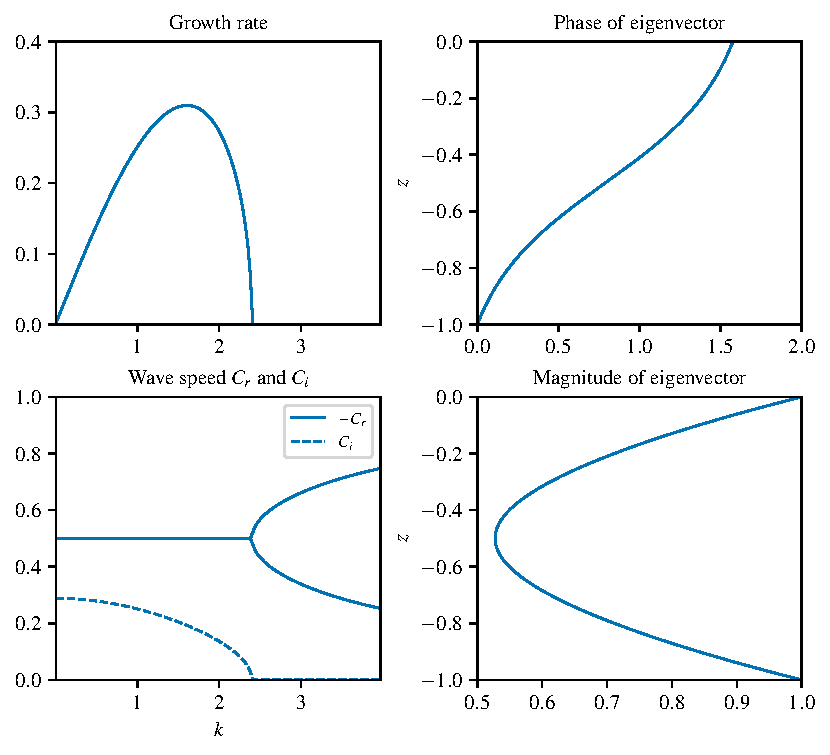
\includegraphics{Eady_matchvallis}
    \caption{Solution to the Eady problem.}
    \label{fig:Eady_matchvallis}
\end{figure}

\begin{figure}
    \centering
    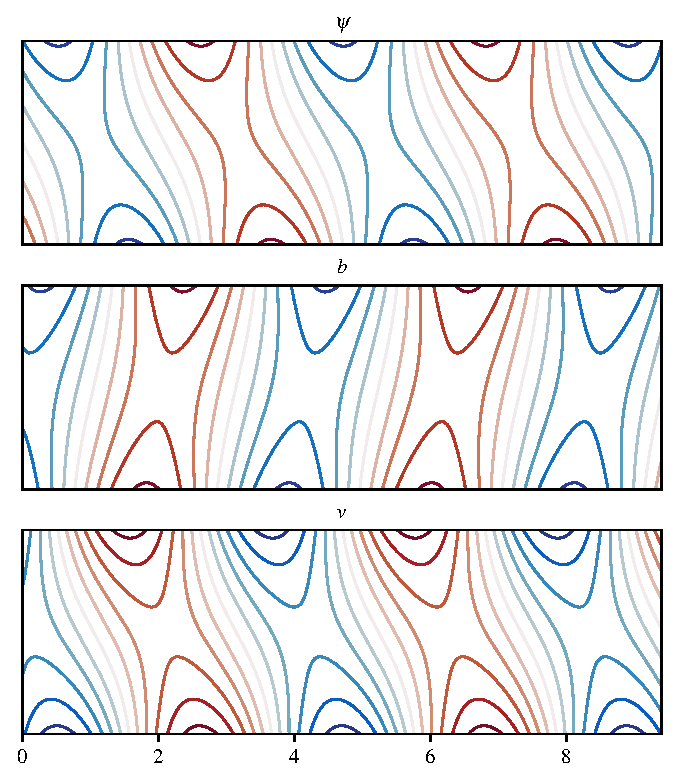
\includegraphics{Eady_profile}
    \caption{Profiles of the most unstable mode for the Eady problem.}
    \label{fig:Eady_profile}
\end{figure}

\section{The ocean Charney instability}
The Eady instability is an instability due to the interaction of two surface modes. We explore the effects of the interior PV gradient by studying the ocean Charney instability \parencite{CapetEtAl_16}. To begin, the ocean Charney instability is due to interaction between the top boundary and the interior. From the Charney–Stern–Pedlosky (CSP) condition, we know that for instability, we need $Q_y$ is the opposite sign to $U_z$ at the upper boundary \parencite[p. 351]{Vallis_17}. For the ocean, there are two ways for this to happen. For an eastward sheared top mean current $U_z>0$, we need $Q_y<0$. For this, we need the curvature of the zonal velocity to overwhelm the positive planetary PV gradient $\beta$. Now if the top mean current is westward sheared $U_z<0$, we need $Q_y>0$ which can be provided by the planetary PV gradient $\beta$. Both can happen in the ocean according to the global study of \cite{TullochEtAl_11}. We study the linear instability of both scenarios. For that, we ignore the bottom boundary by setting $b=0$ at $z=-H$.

\subsection{Idealized profiles inspired by the ocean}
For our preliminary examples to demonstrate Dedalus, we use idealized nondimensional profiles. Converting the code to take real data would be simple. 

The 3DQG system above only needs stratification $N^2(z)$ and mean velocity $U(z)$ at vertical profiles as inputs. That is the data our data will take. We will use exponential stratification
\begin{align}
    N^2(z) = N^2 e^{z/\delta} \qdt{w/} \delta=0.2.
\end{align}
For velocity we use
\begin{align}
    U(z) = (1+z-\delta)e^{z/\delta}/5.
\end{align}
We scale the velocity so that $\dsp{\frac{\pe}{\pe z}\left(\frac{f^2}{N^2}\frac{\pe\psi}{\pe z}\right)}=1$. 

\subsection{Condition for instability}
Note that in our nondimensionalization, the velocity is fixed. To compare the different cases of velocity shear, we flip the sign of $\beta$ instead by using different signs of $\xi^{-2}$. To satisfy the CSP condition, we always need 
\begin{align}
    Q_y = \{\xi^{-2}\}-1<0.
\end{align}
Therefore we need
\begin{align}
    \{\xi^{-2}\}<1.
\end{align}
Note that this means all westward mean velocity is unstable, while eastward velocity has to be strong enough to be unstable. This matches our intuition.

Indeed, Figure \ref{fig:Charney_evalparam} shows the growth rate for select values of $\xi^{-2}$. We see that $\{\xi^{-2}\}=1$ is stable. Other values of $\{\xi^{-2}\}$ show scale selective instability typical of baroclinic instability.

\begin{figure}
    \centering
    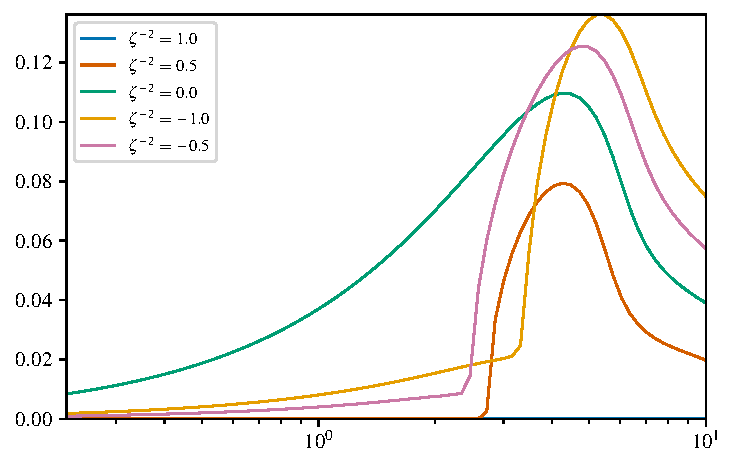
\includegraphics{Charney_evalparam}
    \caption{Growth rate of Charney instability. The $x$-axis is the zonal wavenumber.}
    \label{fig:Charney_evalparam}
\end{figure}

\subsection{Instability profiles}
We pick the two cases of $\{\xi^{-2}\}=\pm0.5$ to look at the profile of the instability. Note that $\{\xi^{-2}\}$ is eastward. Figure \ref{fig:Charney_evecmag} shows the magnitude of the eigenvector of the fastest growing mode, a common value of interest for baroclinic instability. Figure \ref{fig:Charney_instabprofile_west} and \ref{fig:Charney_instabprofile_east} shows some physical variables of the most unstable wavenumber for the westward and eastward case, respectively. We see that the streamfunctions $\psi$ and meridional velocity $v$ lean against the mean flow (note that for these two plots, we actually reserve the mean flow and keep $\beta$ unchanged). They are also out of phase, typical of baroclinic instability.

\begin{figure}
    \centering
    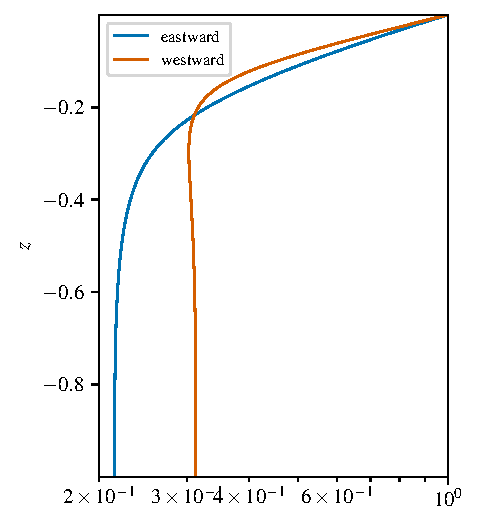
\includegraphics{Charney_evecmag}
    \caption{The magnitude of the eigenvector of the fastest growing mode.}
    \label{fig:Charney_evecmag}
\end{figure}

\begin{figure}
    \centering
    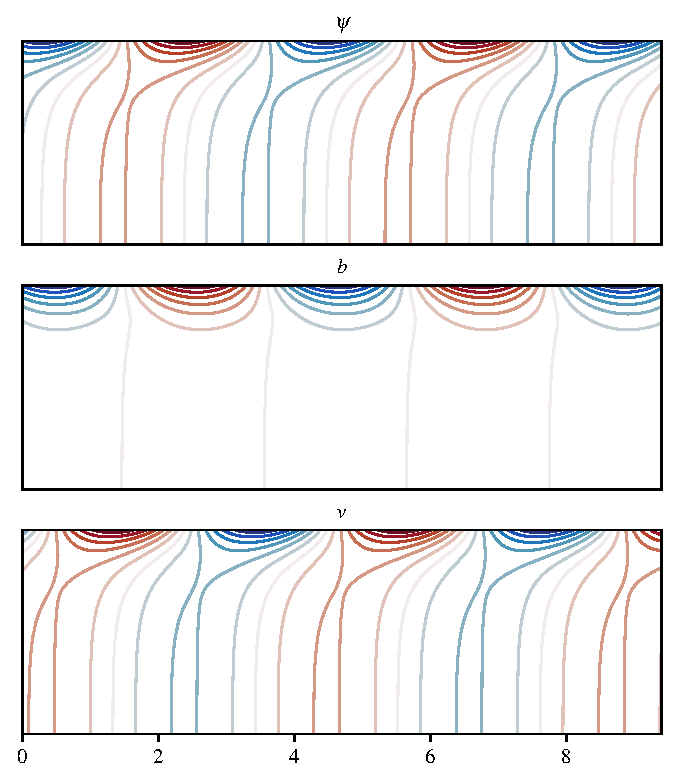
\includegraphics{Charney_instabprofile_west}
    \caption{Physical variables of the most unstable wavenumber for the westward case.}
    \label{fig:Charney_instabprofile_west}
\end{figure}

\begin{figure}
    \centering
    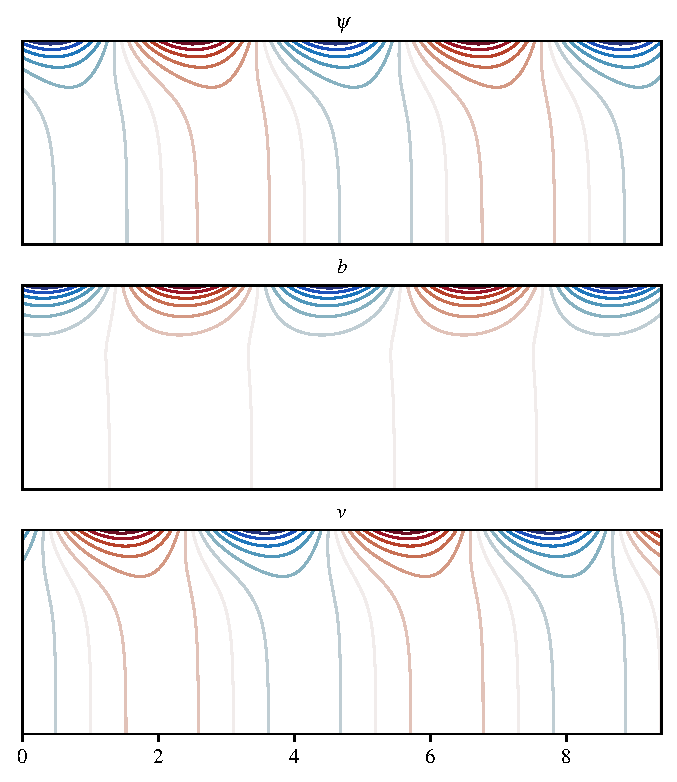
\includegraphics{Charney_instabprofile_east}
    \caption{Same as Figure \ref{fig:Charney_instabprofile_west} but for the eastward case.}
    \label{fig:Charney_instabprofile_east}
\end{figure}

\section{Some comments}
\cite{LuoCallies_23} has code to do linear instability analysis in Dedalus v2. 